% https://www.overleaf.com/latex/templates/sprint-beyond-the-book-template/kgckkccxfxcj
% 這份文件是用上面網址裡的資料建立的
% 2025-02-16 轉換衛教檔案成為 latex format. 


\documentclass[nols]{tufte-book}
%\documentclass{tufte-handout}
\usepackage[caption=false]{subfig}

\usepackage{booksprint}

\setcounter{secnumdepth}{3}
\setcounter{tocdepth}{1}

\usepackage{pdfpages}


\usepackage{fancyhdr}
% 加上 table in the header 
% https://tex.stackexchange.com/questions/113240/tables-as-header-and-footer

% 設定頁碼樣式
\fancypagestyle{plain}{%
  \fancyhf{}
  \fancyfoot[C]{\thepage}
  \renewcommand{\headrulewidth}{0pt}
  \renewcommand{\footrulewidth}{0pt}
}
\fancyfoot[C]{\normalfont\small\thepage}


\usepackage{hyperref} %加入 hyperlink

\usepackage{natbib}

%\usepackage[utf8]{inputenc}
\usepackage[T1]{fontenc}
\usepackage{fontspec}
\renewcommand{\allcapsspacing}[1]{{\addfontfeature{LetterSpace=10.0}#1}}
\renewcommand{\smallcapsspacing}[1]{{\addfontfeature{LetterSpace=5.0}#1}}
\renewcommand{\textsc}[1]{\smallcapsspacing{\textsmallcaps{#1}}}
\renewcommand{\smallcaps}[1]{\smallcapsspacing{\scshape\MakeTextLowercase{#1}}}
% https://www.overleaf.com/latex/examples/demonstration-of-noto-serif-cjk-and-noto-sans-cjk-fonts/sgrwgcddtqsq
\usepackage{setspace}


%set-up 中文環境
\usepackage[CJKspace]{xeCJK}
\usepackage{xpinyin}

\setmainfont{Noto Serif Light}
\setsansfont{Noto Sans}
\setmonofont[Scale=MatchLowercase]{Noto Mono}

\setCJKmainfont{Noto Serif CJK TC}
\setCJKsansfont{Noto Sans CJK TC}
\setCJKmonofont{Noto Sans Mono CJK TC}


%表格
\usepackage{amsmath}
\usepackage{amssymb}
\usepackage{hyperref}
\usepackage{array}

\usepackage{tabularx}
\usepackage{multirow}

\usepackage{ragged2e}
\usepackage{longtable}

\begin{document}
\pagenumbering{roman}


\title[心血管中心衛教手冊]{
\logos
\textbf{心臟衰竭\\
整合性衛教手冊\\
新竹臺大分院心血管中心}}
\author{心血管中心 電話：(03)5326151-525001}
\date{\today}

% 這邊是加上標題頁! 
% 不然 TufteBook會出不來 title page. 

\includepdf[pages=-,offset=-0.5cm 0cm]{title page cv rehab.pdf}


\tableofcontents

\onehalfspacing


\chapter*{前言}
先生、女士您好：
住院期間將啟動心臟衰竭照護及衛教計畫，依個別性照會營養師、物理治療師、藥師等，提供衛教指導，若有疑問請隨時與醫護團隊反應；個管師將於出院後3日內電訪，追蹤返家適應情形，若有相關問題可於電訪中詢問。

\thispagestyle{plain}

\pagenumbering{arabic}
\setcounter{page}{1}


\chapter*{查檢表}
\begingroup
\small
\begin{longtable}{|l|p{6cm}|p{4cm}|}
\hline
\multicolumn{3}{|c|}{\textbf{心臟衰竭衛教查檢表}} \\
\hline
\textbf{項目} & \textbf{內容/聯絡方式} & \textbf{執行者 / 日期} \\
\hline
\endfirsthead

\hline
\multicolumn{3}{|c|}{\textbf{心臟衰竭衛教查檢表（續）}} \\
\hline
\textbf{項目} & \textbf{內容/聯絡方式} & \textbf{執行者 / 日期} \\
\hline
\endhead

\hline
\endfoot

\textbf{【自我管理】} & 29247385  (08:30-12:00; 14:00-17:00)  & 心衰個管師 / 日期 \\
\hline
 & □ 心臟衰竭簡介 & \\
 & □ 心衰日常照護須知 & \\
 & □ 心衰治療注意事項 & \\
 & □ 返家緊急狀況處置 & \\
 & □ 其他： & \\
\hline
\textbf{【心肺復健】} & 523513 (08:30-12:00; 14:00-17:00) & 物理治療師 / 日期 \\
\hline
 & □ 第一期心肺復健 / 危險分級 & \\
 & □ 居家復健計畫說明 & \\
 & □ 臨床諮詢指導 & \\
 & □ 第二期心肺復健計畫 & \\
 & □ 其他： & \\
\hline
\textbf{【營養評估】} & 524304 (08:00-17:00) & 營養師 / 日期 \\
\hline
 & □ 營養評估 / 飲食評估 & \\
 & □ 飲食建議 / 共病控制教育 & \\
 & □ 臨床諮詢指導 & \\
 & □ 其他： & \\
\hline
\textbf{【藥物控制】} & 藥物諮詢專線：524102 (08:30-17:30) & 藥師 / 日期 \\
\hline
 & □ 用藥評估 / 共病控制教育 & \\
 & □ 臨床諮詢指導 & \\
 & □ 其他： & \\
\hline
\textbf{【戒菸衛教】} & 523734 (08:30-17:00) & 戒菸個管師 / 日期 \\
\hline
 & □ 煙癮評估 / 戒菸衛教 & \\
 & □ 戒菸藥物諮詢 & \\
 & □ 無抽菸史，□ 已戒菸 & \\
\hline
\textbf{病人簽收} & & \\
\hline
\end{longtable}
\endgroup


\marginnote[-18cm]{這份查檢表是協助同事們追蹤衛教進度用。家屬們也可以理解整體病患需要衛教的部份有哪些。請注意: 不是每一位病患都需要接受全部的衛教，也不是全部的衛教都要作完才能夠出院，因為出院後一樣可以將衛教完成。}


\section*{目的}

\begin{figure}
    %\centering
    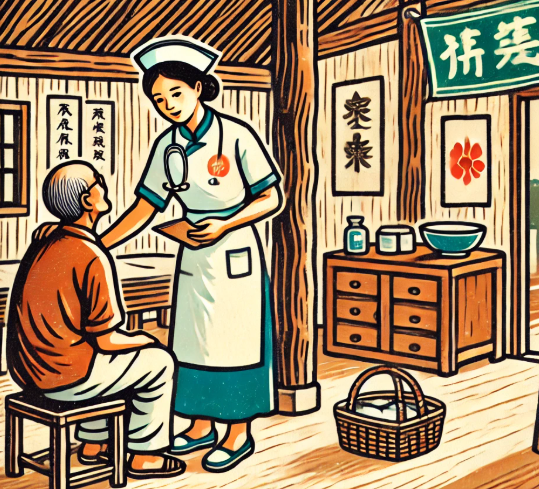
\includegraphics[width=1.0\linewidth]{images/rehab/fig cv rehab education nurse.png}*{醫療上，團隊溝通的重要性: 團隊不是只有醫師，在新竹台大分院，我們有完整的跨團隊合作模式，如果您發現不認識的醫護同仁，來關心您，而且發現他/她對您的病情很了解，請不用緊張喔!}
    \caption{因為人力關係，我們還作不到居家訪視，但是這個是未來期待的目標。}
    \label{images/rehab/fig cv rehab education nurse}
\end{figure}

\chapter{物理治療-心臟復健運動}

心臟復健是對患有心臟疾病的病人，進行規律運動訓練。訓練過程中物理治療師會監控病人的心跳、血壓、血氧與臨床徵候，以求達到增加心肺耐力或體適能來回復正常生活活動及職場所需。\textbf{心臟復健分為三期}：

\begin{itemize}
  \item \textbf{第一期}是住院期及轉銜期(約4-6週)
  \item \textbf{第二期}是門診復健期(約3-6個月)
  \item \textbf{第三期}是維持期(病人居家自行維持心臟復健運動)
\end{itemize}

\textbf{文獻統計資料顯示：有進行心臟復建的心臟衰竭病人，可降低死亡率與再住院率達35\%。}

\begin{longtable}{p{0.15\textwidth}p{0.85\textwidth}}
\caption{進行心臟復健的好處} \label{tab:benefits} \\
\hline
\textbf{編號} & \textbf{好處說明} \\
\hline
\endfirsthead

\multicolumn{2}{c}{\tablename\ \thetable{} -- 續上頁} \\
\hline
\textbf{編號} & \textbf{好處說明} \\
\hline
\endhead

\hline
\multicolumn{2}{r}{續下頁} \\
\endfoot

\hline
\endlastfoot

1 & 降低再住院率 \\
\hline
2 & 降低死亡率 \\
\hline
3 & 減低心臟病危險因子 \\
\hline
4 & 降低膽固醇 \\
\hline
5 & 協助控制血糖、血壓 \\
\hline
6 & 放鬆心情 \\
\hline
7 & 增強心肺耐力 \\

\end{longtable}



\newpage
\section*{運動計畫}
\begin{itemize}
  \item 有氧運動，如：步行、騎腳踏車等；先做間歇式運動，再慢慢增加時間，以達到連續運動20到30分鐘為目標。
  \item 肌力訓練：上肢及下肢抗重力或阻力運動，可做10-15下/組，重複2-3組。
\end{itemize}

\section*{須減緩或停止活動的情況}
\begin{enumerate}
  \item 胸痛、心絞痛、氣喘、呼吸困難、頭暈目眩、噁心嘔吐、臉色發白、發紺等
  \item 身心疲勞或肌肉痠痛無力
  \item 不適當的心跳或血壓反應：出院初期，運動時每分鐘心跳超出休息時的20下以上，或運動後心跳低於休息時心跳10下；收縮壓大於200mmHg，舒張壓大於110mmHg
\end{enumerate}

\section*{適當的運動強度應為}
適度流汗、呼吸增快、短暫且非不愉快的疲累，同時能與人維持正常談話。

\section*{活動注意事項}
\begin{itemize}
  \item 避免推、拉、抬、舉重物與憋氣用力的活動以減少對心臟的負荷。
  \item 避免溫度過高、過低或濕度過高的地方活動。
  \item 勿從事競賽型活動。
  \item 運動必須包含5至10分鐘的暖身及緩和活動。
  \item 運動時間，為飯後1至2小時後，且飯前避免食用刺激性食物。
  \item 感冒及身心疲勞請勿運動。
\end{itemize}


\newpage
\section*{線上影音復健資源}

\begin{figure}
    \centering
    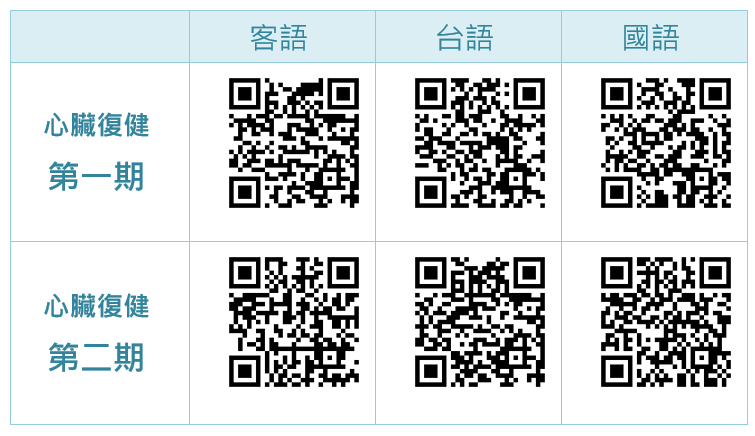
\includegraphics[width=1\linewidth]{images/rehab/fig_cardiac rehab QR code.png}
    \caption{心肺復健第一、二期衛教影片的QR code連結}
    \label{images/rehab/fig_cardiac rehab QR code}
\end{figure}

\chapter{飲食注意事項}
\begin{longtable}{|p{0.2\textwidth}|p{0.8\textwidth}|}
\caption{心衰竭患者的營養建議與注意事項} \label{tab:nutrition} \\
\hline
\textbf{主題} & \textbf{內容說明} \\
\hline
\endfirsthead

\multicolumn{2}{c}{\tablename\ \thetable{} -- 續上頁} \\
\hline
\textbf{主題} & \textbf{內容說明} \\
\hline
\endhead

\hline
\multicolumn{2}{r}{續下頁} \\
\endfoot

\hline
\endlastfoot

基本原則 & 良好的營養狀況有助於心衰竭患者維持病況，適當的攝取身體所需要的熱量及營養素能保護患者心臟及維持較佳的健康狀況。建議和營養師討論每日的熱量及營養需求。當食慾下降及進食量減少時，建議以少量多餐的方式進食。另外，可考慮補充適當的「濃縮營養品」，補足攝取的不足。 \\
\hline

低鈉飲食說明 & 鈉離子在人體中主要負責調控體內水分的平衡。過多的「鈉」離子會使身體水份累積、高血壓、肺積水、增加心臟的負荷。鈉離子廣泛存在於食物中，是鹽、味精、蕃茄醬、豆瓣醬、味噌、咖哩、干貝醬等\textbf{調味料}的主要成分之一。 \\
\hline

低鈉食物選擇與烹飪技巧 & 
\begin{itemize}
\item 建議每日限鹽\textbf{3公克（1200毫克鈉）至5公克（2000毫克鈉）}
\item 選擇天然食材，以新鮮食物本身的原味為主
\item \textbf{避免加工、罐頭及醃製、滷製食品}
\item 忌鈉含量高加工食品
\item 多善用天然食材的香氣調味
\item \textbf{減少鈉含量高的調味料使用}
\item 注意市售低鈉產品的成分
\item 閱讀包裝食品的「鈉」含量標示
\end{itemize} \\
\hline

外食減鹽技巧 & 
\begin{itemize}
\item 飯類：避免加鹽與醬油烹煮的飯類、不額外淋滷肉汁或菜湯
\item 麵類：建議選擇湯麵但是不喝湯、選擇水煮水餃，不再沾醬料，可沾白醋。若菜餚醬料過多過鹹，可以熱水涮洗過再吃。
\end{itemize} \\
\hline

水分控制原則 & 體內過多的水份易增加心臟的負荷，可能會出現水腫或呼吸急促等症狀，需遵循醫囑控制每日水分攝取。 \\
\hline

水分控制技巧 & 
\begin{itemize}
\item \textbf{每日起床排尿後用餐前}稱重，\textbf{逐日記錄體重}
\item 計算固體食物中的水分含量
\item 使用固定容器盛裝飲水
\item \textbf{避免攝取過多湯汁、飲料等}
\item 注意高含水量食物的攝取量
\end{itemize} \\
\hline

解渴小技巧 & 
\begin{itemize}
\item \textbf{用開水漱口，再將水吐出}
\item 可以口含冰塊或檸檬汁冰塊（需納入水分計算）
\item 咀嚼清涼口香糖或喉糖
\item 使用護唇膏保持嘴唇濕潤
\end{itemize} \\

\end{longtable}

\begin{figure}
    \centering
    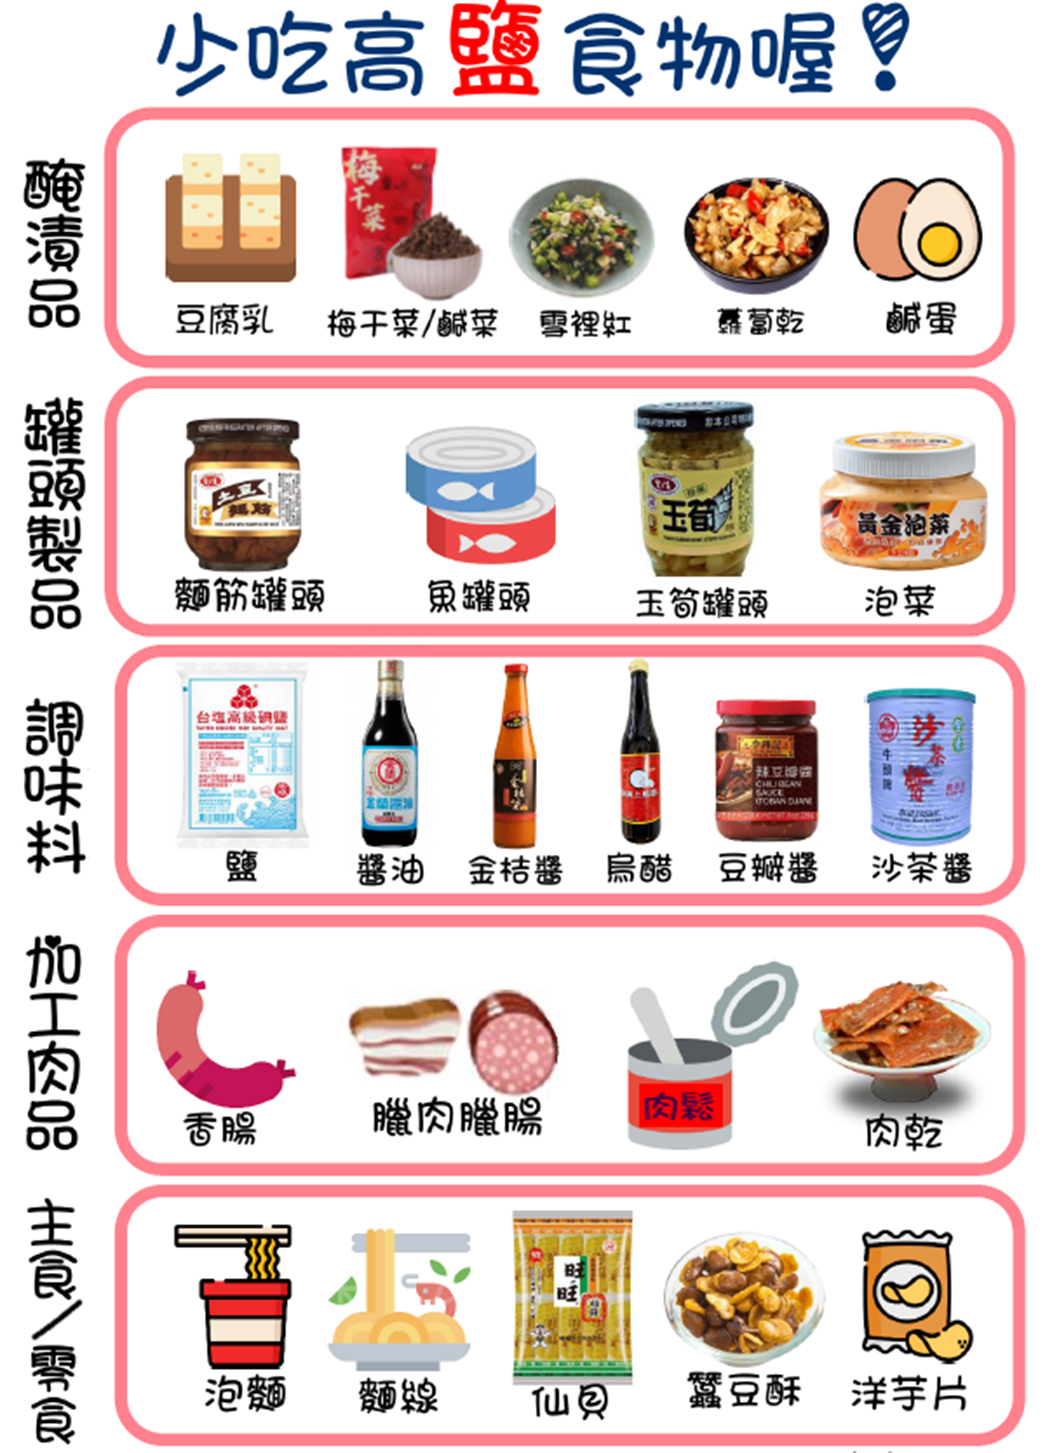
\includegraphics[width=1\linewidth]{images/rehab/fig_cardiac rehab diet.png}
    \caption{飲食小重點: 要注意的事項}
    \label{images/rehab/fig_cardiac rehab diet}
\end{figure}


\chapter{戒菸-我想戒菸有什麼方法？}
\begin{longtable}{|p{0.3\textwidth}|p{0.7\textwidth}|}
\caption{戒菸衛教資訊} \label{tab:smoking} \\
\hline
\textbf{主題} & \textbf{說明內容} \\
\hline
\endfirsthead

\multicolumn{2}{c}{\tablename\ \thetable{} -- 續上頁} \\
\hline
\textbf{主題} & \textbf{說明內容} \\
\hline
\endhead

\hline
\multicolumn{2}{r}{續下頁} \\
\endfoot

\hline
\endlastfoot

吸菸危害 & 
\begin{itemize}
\item 加重心臟負擔並加速病情惡化
\item 尼古丁和一氧化碳會收縮血管、升高血壓
\item 促進動脈粥狀硬化，加劇心肌缺氧
\item 降低藥物治療效果
\item 增加住院率與死亡率
\end{itemize} \\
\hline

戒菸效益 & 
\begin{itemize}
\item 顯著改善心衰竭患者的預後
\item 減少併發症
\item 提升生活品質
\end{itemize} \\
\hline

現況分析 & 研究調查顯示，吸菸者有70\%曾嘗試戒菸，但未經由專業協助，短期戒菸成功率不到10\%。需要配合戒菸專業輔導機構與正確使用輔助藥物，以提高戒菸成功率。 \\
\hline

\multicolumn{2}{|c|}{\textbf{戒菸明星(STAR)計畫}} \\
\hline

S (Set) & 慎重設定戒菸日，2週內！ \\
\hline

T (Tell) & 公開決心，爭取支持，昭告眾親朋好友！ \\
\hline

A (Anticipate) & 預期戒菸過程可能會遇到的困難！認識戒斷症候群，詳讀。 \\
\hline

R (Remove) & 移除引起吸菸念頭的一切及用品。 \\
\hline

補充說明 & 本院備有戒菸教戰手冊「戒菸教戰手冊」，歡迎索取。 \\

\end{longtable}


\newpage
\section*{戒菸方法比較}


\begin{longtable}{|p{0.12\textwidth}|p{0.22\textwidth}|p{0.22\textwidth}|p{0.22\textwidth}|p{0.22\textwidth}|}
\caption{戒菸方式比較表} \label{tab:smoking-comparison} \\
\hline
\textbf{項目} & \textbf{靠意志力戒菸} & \textbf{戒菸諮詢} & \textbf{戒菸藥物} & \textbf{戒菸藥物+諮詢} \\
\hline
\endfirsthead

\multicolumn{5}{c}{\tablename\ \thetable{} -- 續上頁} \\
\hline
\textbf{項目} & \textbf{靠意志力戒菸} & \textbf{戒菸諮詢} & \textbf{戒菸藥物} & \textbf{戒菸藥物+諮詢} \\
\hline
\endhead

\hline
\multicolumn{5}{r}{續下頁} \\
\endfoot

\hline
\endlastfoot

選項要做的事 & 
\begin{itemize}
\item 絕對不吸菸
\item 環境沒有菸
\item 告知週遭自己要戒菸
\item 想抽菸時，想戒菸理由
\end{itemize} & 
到提供戒菸服務的醫事機構 \newline
台大新竹醫院戒菸(03)5326151 轉 523551 或 523734 & 
同戒菸諮詢 & 
同戒菸諮詢 \\
\hline

成功率 & 3-5\% & 
24.4\% \newline
(低度菸癮戒菸成功率) & 
25.2\% \newline
(中高度菸癮以上戒菸成功率) & 
27.6\% \newline
(中高度菸癮以上戒菸成功率) \\
\hline

優缺點 & 
\begin{itemize}
\item 省時間，不需前往醫院或打電話
\item 不需額外花錢
\item 菸癮越大戒菸越難成功
\end{itemize} & 
\begin{itemize}
\item 容易看見找出並解決戒菸
\item 菸癮重的人較難成功
\item 需付出額外時間
\end{itemize} & 
\begin{itemize}
\item 降低吸菸的衝動
\item 緩解戒菸時身體不適
\item 菸癮低的人幫助不大
\item 使用藥物不同，有不同副作用
\item 需固定用藥
\end{itemize} & 
\begin{itemize}
\item 成功率高，可同時處理身體、心理、社交問題
\item 菸癮低的人不需用藥
\item 依使用藥物不同，有不同副作用
\item 需固定用藥
\item 付出額外時
\end{itemize} \\
\hline


如何執行？ & 
\begin{enumerate}
\item 設立目標(2週內)
\item 告知親朋好友
\item 移除周遭環境菸品
\item 使用轉移注意力技巧
\end{enumerate} & 
\multicolumn{3}{p{0.66\textwidth}|}{
  \begin{minipage}{\linewidth}
    {\small
      1. 台大新竹醫院戒菸 (03)5326151 轉 523551 或 523734 \newline
      2. 撥打(0800-636363 戒菸專線) \newline
      3. 網路預約戒菸門診 https://www.hch.gov.tw
    }
  \end{minipage}
} \\
\hline

限制條件 & 無 & 無 & \multicolumn{2}{p{0.44\textwidth}|}{健保且滿 18 歲才有補助。僅適用於每天吸菸量 10 根以上，或成癮度 4 分(含)以上} \\

\end{longtable}




\chapter{藥物注意事項}
\begin{longtable}{|p{0.3\textwidth}|p{0.7\textwidth}|}
\caption{心臟衰竭用藥注意事項} \label{tab:medication} \\
\hline
\textbf{項目} & \textbf{說明} \\
\hline
\endfirsthead

\multicolumn{2}{c}{\tablename\ \thetable{} -- 續上頁} \\
\hline
\textbf{項目} & \textbf{說明} \\
\hline
\endhead

\hline
\multicolumn{2}{r}{續下頁} \\
\endfoot

\hline
\endlastfoot

基本原則 & 心臟衰竭須長期服用藥物，請勿自行停藥，若有服藥的問題，請告知醫師或來電與藥師或專科護理師討論。 \\
\hline

過敏反應處理 & 服藥後，若有嚴重的過敏反應，如呼吸困難、喉頭腫脹、全身紅疹，請立即停藥且就醫。 \\
\hline

用藥資訊告知 & 請告知醫師或藥師所服用的藥品，包含中藥與保健食品，避免自行購買藥物服用（避免使用NSAIDS非類固醇消炎止痛藥）。 \\
\hline

藥物調整原則 & 醫師會依據疾病與症狀調整藥品，請勿自行調整藥物或停用。 \\
\hline

監測建議 & 建議服用藥物前，先監測血壓、心跳。請維持每日測量血壓、心跳、體重的習慣，血壓監測口訣722（每日2次，每次2下，一周7次）。 \\
\hline

\multicolumn{2}{|l|}{\textbf{若忘記吃藥時，我應該...}} \\
\hline

服藥時間範例 & 若固定每日早上9點服用藥物 \\
& 
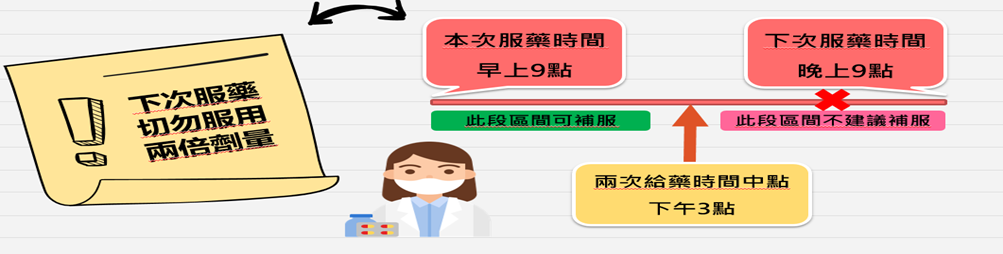
\includegraphics[width=1\linewidth]{images/rehab/fig_medication skip education.png}
\\

\end{longtable}

\section*{藥物介紹}
\begin{figure}
    %\centering
    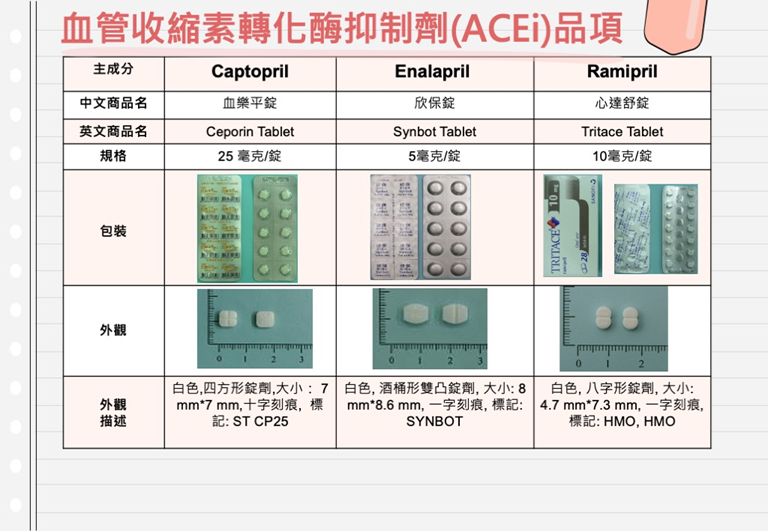
\includegraphics[width=1\linewidth]{images/cv-med/fig cv med ACEi.png}*{血管張力素轉化酶抑制劑(ACE-I/)/血管張力素II 受體抑制劑(ARB)： 
作用：降低血壓，具保護心臟、長期使用可降低死亡率、急性冠心症發作與心衰竭的風險。
注意事項：監測血壓。懷孕與哺乳者應避免使用。}
    \caption{Angiotensin-converting enzyme inhibitor, ACEi. }
    \label{fig:enter-label}
\end{figure}

\begin{figure}
    %\centering
    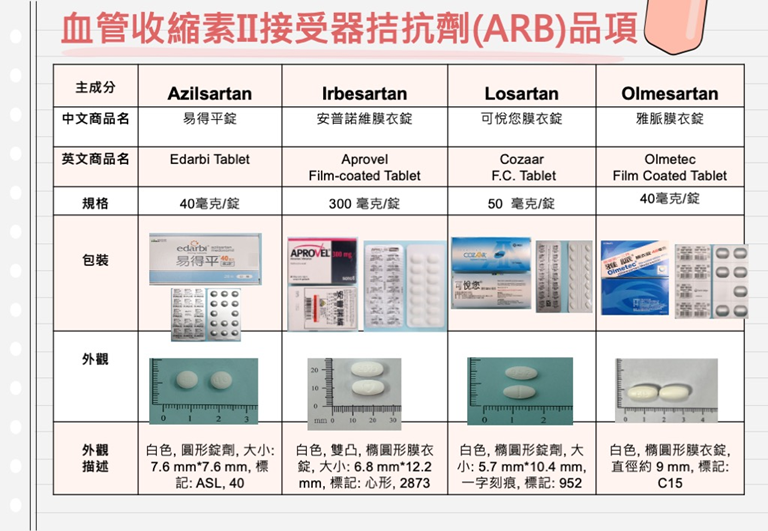
\includegraphics[width=1\linewidth]{images/cv-med/fig cv med ARB 1.png}
    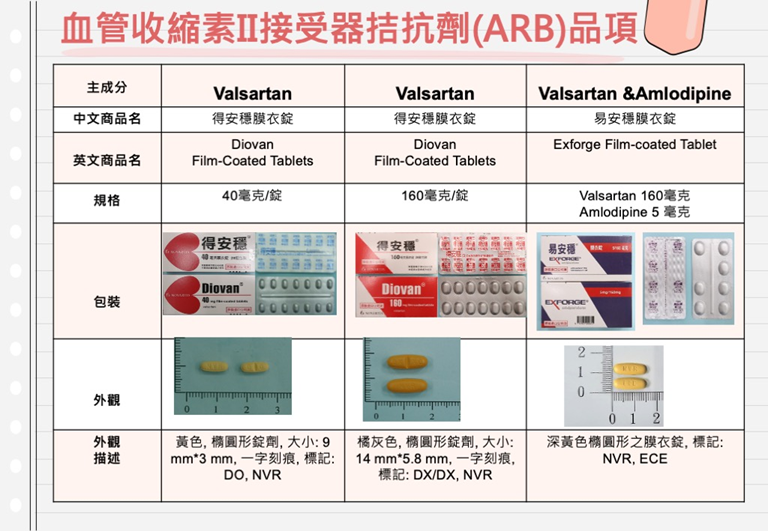
\includegraphics[width=1\linewidth]{images/cv-med/fig cv med ARB 2.png}*{血管張力素轉化酶抑制劑(ACE-I/)/血管張力素II 受體抑制劑(ARB)： 
作用：降低血壓，具保護心臟、長期使用可降低死亡率、急性冠心症發作與心衰竭的風險。
注意事項：監測血壓。懷孕與哺乳者應避免使用。
}
    \caption{Angiotensin receptor blocker, ARB. }
    \label{images/cv-med/fig cv med ARB}
\end{figure}


\begin{figure}
    %\centering
    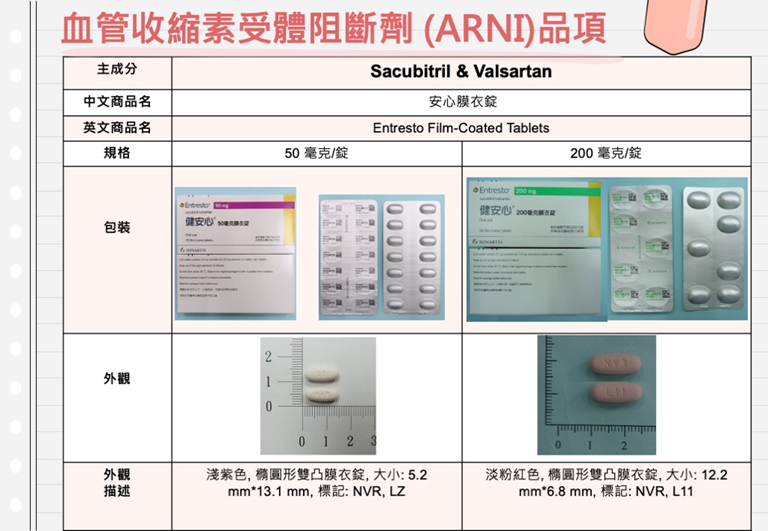
\includegraphics[width=1\linewidth]{images/cv-med/fig cv med ARNI.png}*{血管張力素受體-腦啡肽酶抑制劑(ARNI)： 作用：治療慢性心臟衰竭（紐約心臟學會[NYHA]第二級至第四級）且左心室射出分率降低的病人，減少心血管死亡和心臟衰竭住院風險。
注意事項：監測血壓。懷孕與哺乳者應避免使用。
}
    \caption{Angiotensin receptor neprilysin inhibitor, ARNI. }
    \label{images/cv-med/fig cv med ARNI}
\end{figure}

\begin{figure}
    %\centering
    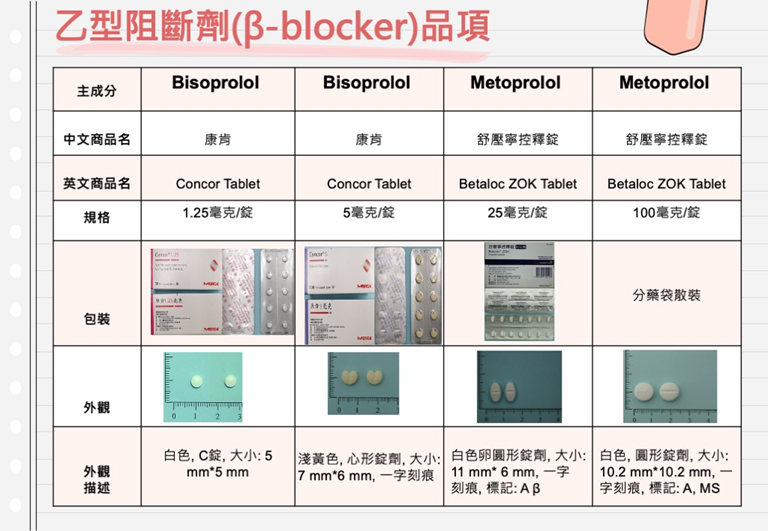
\includegraphics[width=1\linewidth]{images/cv-med/fig cv med BB 1.png}
    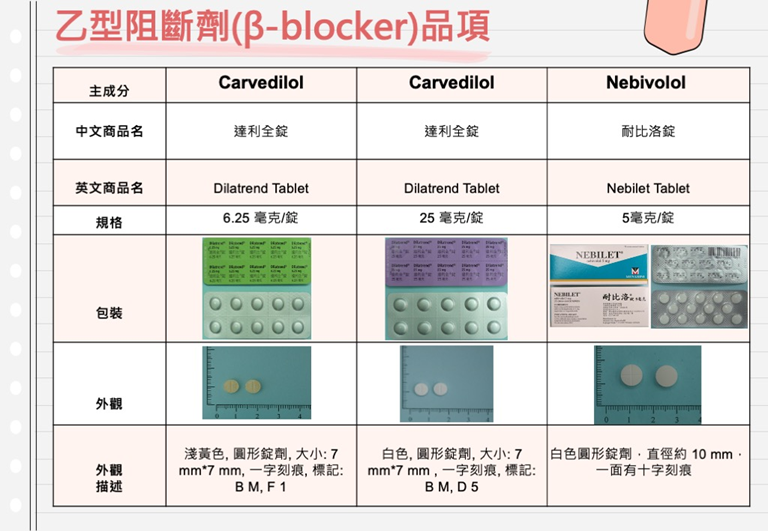
\includegraphics[width=1\linewidth]{images/cv-med/fig cv med BB 2.png}*{乙型阻斷劑 (β -blocker)
作用： 降低心跳且降低血壓、減輕心臟工作負荷，長期可預防心衰竭與降低心因性死亡。
注意事項： 監測心跳與血壓。
}
    \caption{Beta-blocker, BB. }
    \label{images/cv-med/fig cv med BB}
\end{figure}

\begin{figure}
    %\centering
    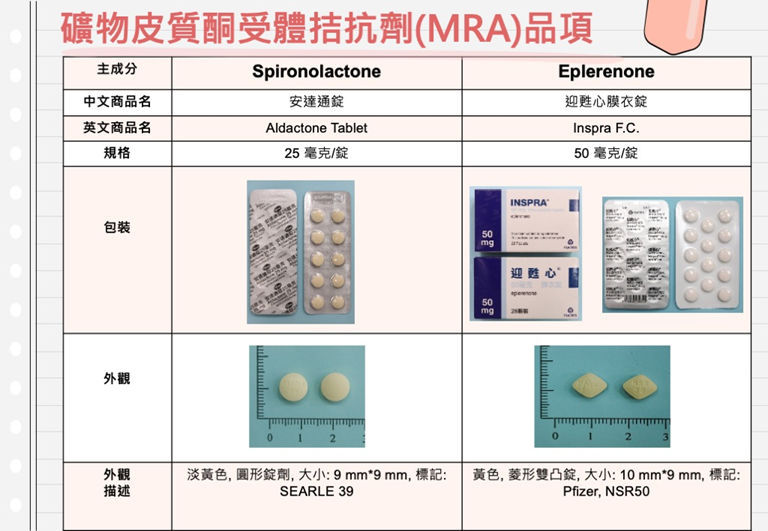
\includegraphics[width=1\linewidth]{images/cv-med/fig cv med MRA.png}*{作用： 降低死亡率與再住院風險，改善臨床症狀。
注意事項：如果意識模糊、心跳不規則、噁心或嘔吐或四肢無力時，應立即就醫。若出現乳房腫脹疼痛、毛髮增生，請於回診時告知醫生。
}
    \caption{Mineralocorticoid receptor antagonist, MRA. }
    \label{images/cv-med/fig cv med MRA}
\end{figure}

\begin{figure}
    %\centering
    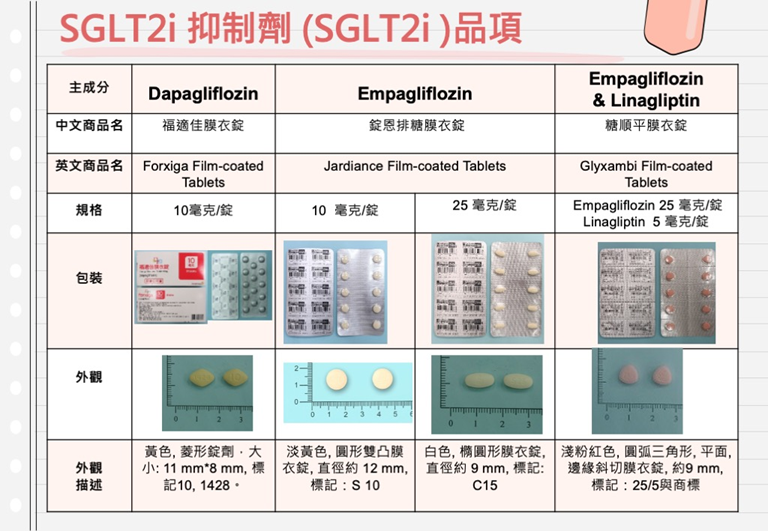
\includegraphics[width=1\linewidth]{images/cv-med/fig cv med SGLT2i.png}*{第二型鈉-葡萄糖轉運通道抑制劑(SGLT2 inhibitor)： 
作用： 可降低心血管死亡、心衰竭住院和心衰竭緊急就醫的風險。
注意事項: 低血糖、泌尿道感染、低血壓或脫水、腎損傷。
}
    \caption{Sodium-glucose co-transporter 2 inhibitor, SGLT2i. }
    \label{images/cv-med/fig cv med SGLT2i}
\end{figure}

\chapter{疫苗接種相關}
\begin{longtable}{|p{0.25\textwidth}|p{0.75\textwidth}|}
\caption{心衰竭患者疫苗接種建議} \label{tab:vaccine} \\
\hline
\textbf{項目} & \textbf{說明} \\
\hline
\endfirsthead

\multicolumn{2}{c}{\tablename\ \thetable{} -- 續上頁} \\
\hline
\textbf{項目} & \textbf{說明} \\
\hline
\endhead

\hline
\multicolumn{2}{r}{續下頁} \\
\endfoot

\hline
\endlastfoot

基本建議 & \textbf{每年接種流感疫苗 + 肺炎鏈球菌疫苗（PCV13 + PPSV23）為心衰竭患者的標準建議}，有助於降低感染、住院與死亡風險。 \\
\hline

\multirow{3}{*}{\textbf{流感疫苗}} & \textbf{建議所有心衰竭病人每年接種流感疫苗} \\ 
\cline{2-2}
& \textbf{流感感染與心衰竭惡化密切相關}，可增加住院與死亡風險 \\
\cline{2-2}
& 研究顯示，流感疫苗可能透過\textbf{降低發炎反應、減少心血管併發症}來提供心臟保護作用 \\
\hline

\multirow{4}{*}{\textbf{肺炎鏈球菌疫苗}} & \textbf{建議所有心衰竭患者接種肺炎鏈球菌疫苗}，特別是 65 歲以上或有其他高風險因素（如糖尿病、慢性腎病） \\
\cline{2-2}
& \textbf{疫苗種類：} \\
& \begin{itemize}
\item \textbf{PCV13（Prevnar 13）}：可先接種，以建立更強的免疫反應
\item \textbf{PPSV23（Pneumovax 23）}：在 PCV13 之後 1 年內接種，以提供更廣泛的保護
\end{itemize} \\
\hline

\multirow{3}{*}{疫苗的潛在好處} & \textbf{減少心衰竭惡化與住院}：超過一半的心衰竭住院與呼吸道感染有關，疫苗有助於減少感染相關的病情惡化 \\
\cline{2-2}
& \textbf{降低心血管事件風險}：疫苗可能透過減少發炎反應、降低血管內皮功能障礙來提供心血管保護 \\
\cline{2-2}
& \textbf{提高存活率}：某些研究顯示，接種流感疫苗的患者死亡率較低 \\

\end{longtable}

\chapter{緊急狀況處置}
\begin{longtable}{|p{0.15\textwidth}|p{0.85\textwidth}|}
\caption{緊急就醫指引：立即返院就診情形} \label{tab:emergency-signs} \\
\hline
\textbf{編號} & \textbf{症狀說明} \\
\hline
\endfirsthead

\multicolumn{2}{c}{\tablename\ \thetable{} -- 續上頁} \\
\hline
\textbf{編號} & \textbf{症狀說明} \\
\hline
\endhead

\hline
\multicolumn{2}{r}{續下頁} \\
\endfoot

\hline
\endlastfoot

1 & \textbf{非常態性}心跳小於50次/分，收縮壓小於100mmg，合併\textbf{頭暈或全身無力疲倦} \\
\hline

2 & \textbf{呼吸困難}，伴隨劇烈咳嗽且有粉紅色泡沫痰 \\
\hline

3 & \textbf{四肢冰冷或發紫} \\
\hline

4 & 不明原因\textbf{昏倒} \\
\hline

5 & \textbf{小便量減少}，下肢水腫與體重一周內快速增加2公斤以上 \\
\hline

\multicolumn{2}{|p{\textwidth}|}{\textbf{注意事項：}以上1-4症狀休息15分鐘症狀仍未改善緩解，或出現5的情形，\textbf{需立即就醫}。} \\

\end{longtable}


% The bibliography style.
%\bibliographystyle{abbrv}
%\bibliography{Reference}

\end{document}